\documentclass{beamer}

\usepackage{graphicx,hyperref,udesc,url}
\usepackage[latin1]{inputenc}
%\usepackage[T1]{fontenc}
\usepackage{booktabs}
\usepackage[portuges]{babel}


\title[A Universidade, a Computa��o e as Barreiras]{A Universidade, a Computa��o \\ e as Barreiras}

\author[Rafael Castro]{
    Rafael Castro\\\medskip
    {\small \url{rafaelcgs10@gmail.com}}}

    \institute[UDESC]{
        Departamento de Ci\^encia da Computa\c{c}\~ao \\
            Centro de Ci\^encias e Tecnol\'ogicas\\
            Universidade do Estado de Santa Catarina}

\date{07/03/2018}

\begin{document}

\begin{frame}
\titlepage

\end{frame}

\begin{frame}
\frametitle{A Universidade - Expectativas}
  \begin{figure}
     \centering 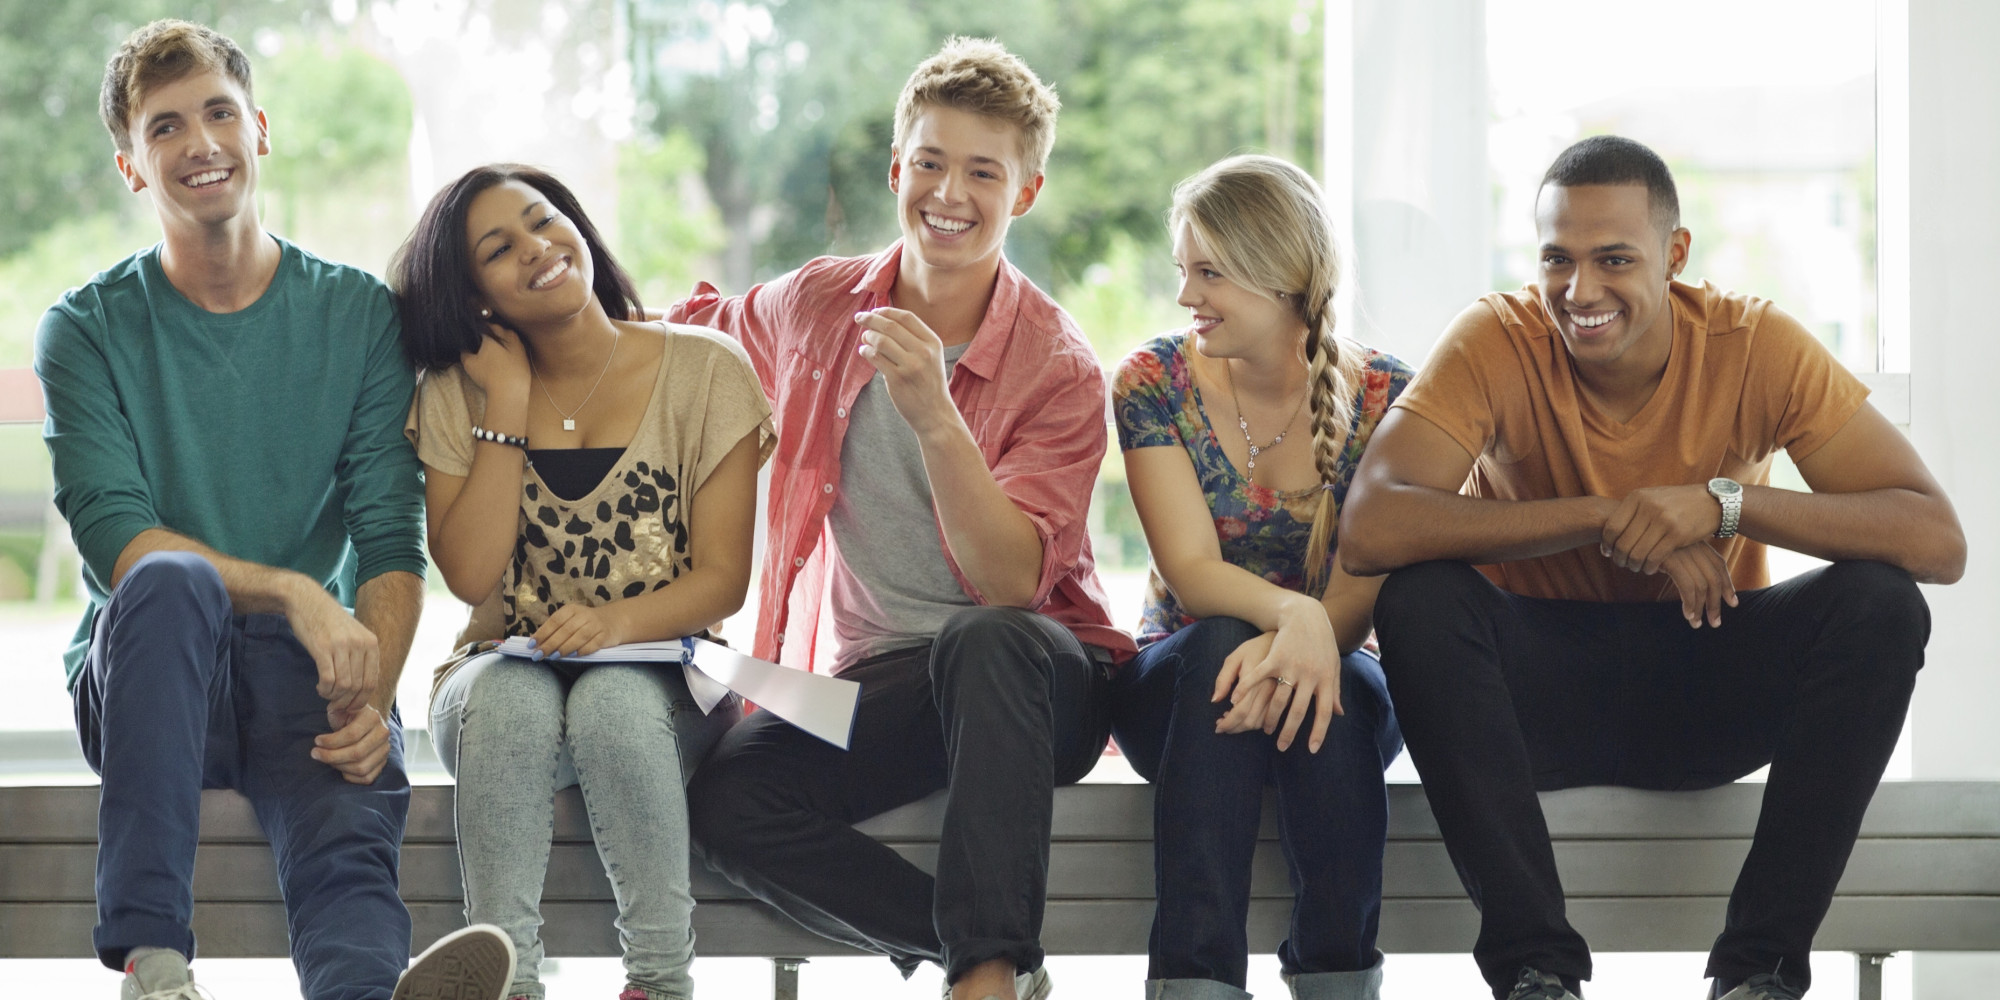
\includegraphics[width=0.9\textwidth]{expetation.jpeg}
  \end{figure}
\end{frame}

\begin{frame}
\frametitle{A Universidade - Realidade}
  \begin{figure}
     \centering 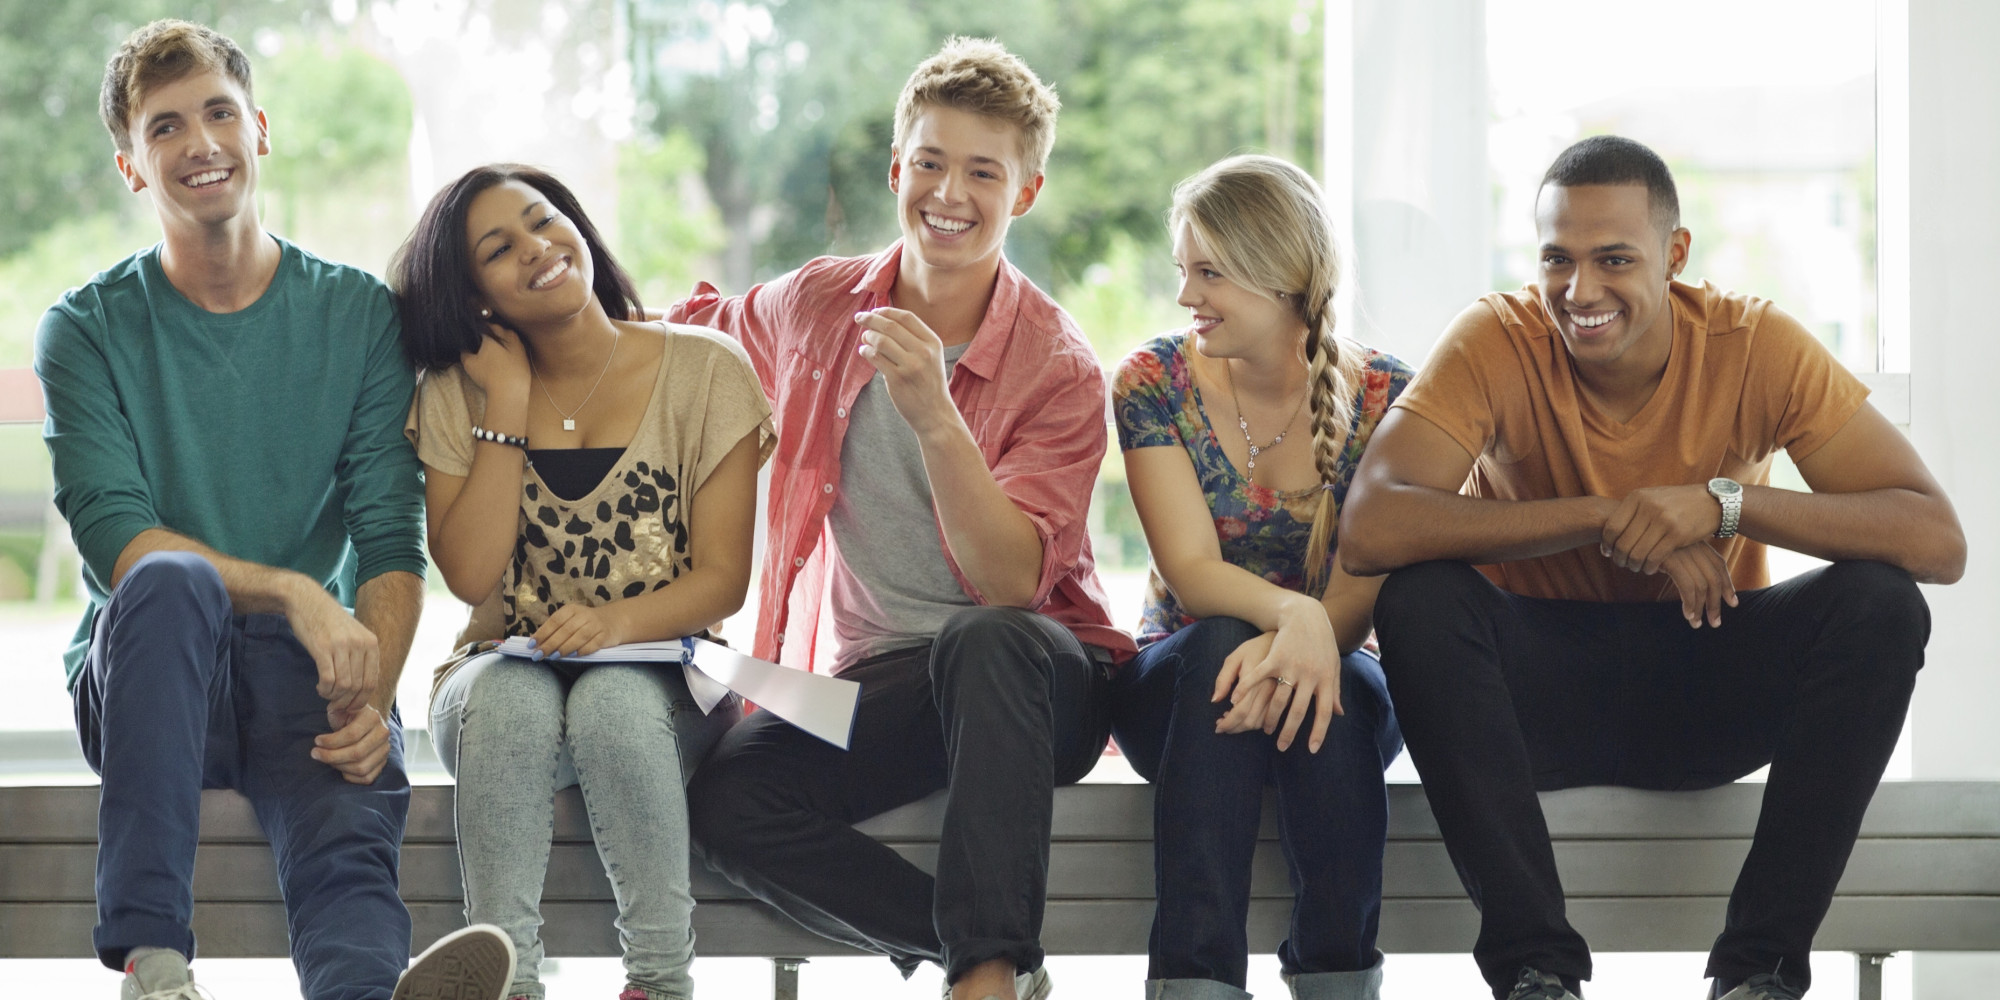
\includegraphics[width=0.9\textwidth]{expetation.jpeg}
  \end{figure}
\end{frame}

\begin{frame}
\frametitle{Motiva��o}
\begin{itemize}
\item A parte infeliz ficou para tr�s, agora � s� estudar o que eu gosto.
\item O foco deste col�quio � a entrada no curso de Ci�ncia da Computa��o.
\item Alta taxa de desist�ncia: ''O curso n�o era o que esperava�� e ''Dificuldade de acompanhar as mat�rias�� com $48\%$ e $24\%$
    , respectivamente, como causas da desist�ncia.
\item \huge{Como sobreviver?}
\end{itemize}
\end{frame}

\section{A Universidade}
\begin{frame}
\frametitle{O que � a universidade?}
    \begin{itemize}
        \item Qual o papel primordial das universidades?
        \item O artigo 207 da constitui��o garante o chamado trip� da universidade, que
            � a indissociabilidade entre ensino, pesquisa e extens�o.
    \begin {itemize}
        \item O ensino acontece por meio das aulas, exerc�cio dos docentes.
        \item A pesquisa � aplica��o dos conhecimentos b�sicos, passado pelos docentes, com a finalidade principal de produzir algo novo.
        \item A extens�o busca articular com a sociedade os conhecimentos desenvolvidos por meio da pesquisa e do ensino.
    \end{itemize}
\end{itemize}
\end{frame}

\begin{frame}
\frametitle{Para que entrar numa universidade?}
    \begin{itemize}
        \item O mito:a universidade serve exclusivamente para  alimentar o mercado de trabalho.
        \item Consequ�ncias:
                \begin{itemize}
                   \item Cria��o de mais universidades particulares.
                   \item Baixo desenvolvimento de pesquisas.
                   \item ''Venda�� de diplomas.
                   \item Fim da meritocracia.
                \end{itemize}
    \end{itemize}
\end{itemize}
\end{frame}
\end{document}
